\documentclass{article}
\usepackage{mainPoly}

\title{Probabilités conditionnelles et indépendance d'événements}
\date{}
\author{Première Spécialité Mathématiques}

\begin{document}
\maketitle

\section{Introduction : Vocabulaire des probabilités}
\begin{tcolorbox}
\textbf{Un joueur ou une joueuse lance deux dés à six faces équilibrés, et observe la somme des valeurs obtenues.}
\end{tcolorbox}
\begin{definition}
\hfill
\begin{itemize}
\item Une telle situation où le résultats possibles sont connus, mais où l'issue n'est a priori pas décidée à l'avance est nommée \textbf{Expérience aléatoire}.
\item L'ensemble des \textbf{issues} possible de cette expérience est nommé l'\textbf{univers}, habituellement noté $\Omega$. (Ici, un univers envisageable pour cette expérience est $\Omega = \{2;3;4;5;6;7;8;9;10;11;12\}$)
\item Un sous-ensemble de l'univers $\Omega$ est appelé \textbf{événement}. (Par exemple, l'événement correspondant à obtenir une somme paire serait $A = \{2;4;6;8;10;12\}$)
\end{itemize}
\end{definition}
\begin{definition}
Soient $A$ et $B$ deux événements d'une expérience aléatoire d'univers $\Omega$.
\begin{itemize}
\item Si $A = \Omega$, $A$ est appelé \textbf{événement certain}. (Par exemple, obtenir un nombre inférieur à $13$ à l'aide de deux dés est un événement certain)
\item Si $A = \emptyset$ (l'ensemble vide), alors $A$ est appelé \textbf{événement impossible}. (Par exemple, obtenir $1$ à l'aide de deux dés est un événement impossible)
\item L'\textbf{union} des événements $A$ et $B$, noté $A \cup B$, se lisant \og $A$ \textbf{union} $B$\fg, est l'événement réalisant les issues de $A$ \textbf{ou} celles de $B$. (Par exemple, si $A = \{4;10\}$ et $B = \{10;12\}$, alors leur union est donnée $A \cup B = \{4;10;12\}$)
\item L'\textbf{intersection} des événements $A$ et $B$ noté $A \cap B$, se lisant \og $A$ \textbf{inter} $B$, est l'évenement réalisant à la fois les issues de $A$ \textbf{et} celles de $B$. (Par exemple, si $A = \{4;10\}$ et $B = \{10;12\}$, alors leur intersection est donnée par $A \cap B = \{10\}$)
\item Le complémentaire de l'événement $A$ noté $\overbar{A}$, se lisant \og $A$ \textbf{barre}\fg, est l'événement réalisant toutes les issues qui ne sont pas réalisées par $A$. (Par exemple, le complémentaire de l'évenement correspondant à obtenir une somme paire serait l'événement correspondant à obtenir une somme impaire)
\end{itemize}
\end{definition}
\begin{center}
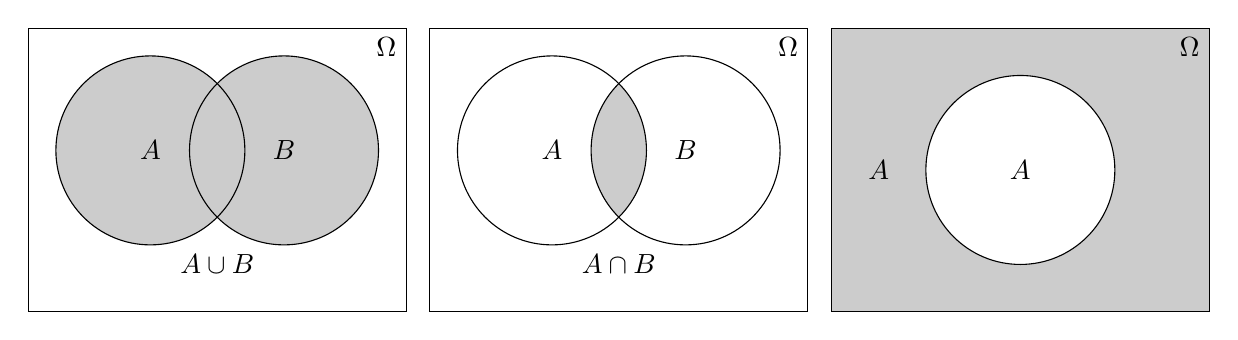
\begin{tikzpicture}[scale = 0.6]
\draw (-4,-2) rectangle (4,4) node[below left] {$\Omega$};
\begin{scope}
\clip (135:2) circle (2);
\fill[color=gray!40] (45:2) circle (2);
\end{scope}
\draw (135:2) node{$A$} circle (2);
\draw (45:2) node{$B$} circle (2);
\draw (0,-1) node{$A \cap B$};
\begin{scope}[xshift=-8.5cm]
\draw (-4,-2) rectangle (4,4) node[below left] {$\Omega$};
\fill[color=gray!40] (135:2) circle (2);
\fill[color=gray!40] (45:2) circle (2);
\draw (135:2) node{$A$} circle (2);
\draw (45:2) node{$B$} circle (2);
\draw (0,-1) node{$A \cup B$};
\end{scope}
\begin{scope}[xshift=8.5cm]
\fill[color=gray!40] (-4,-2) rectangle (4,4);
\draw (-4,-2) rectangle (4,4) node[below left] {$\Omega$};
\fill[color=white] (0,1) circle (2);
\draw (0,1) circle (2) node {$A$};
\draw (-3,1) node {$\overbar{A}$};
\end{scope}
\end{tikzpicture}   
\end{center}
\begin{example}
Proposer deux événements $A$ et $B$ dont l'intersection et l'union sont non-vide.

\emptybox{2cm}
\end{example}
\newpage
\begin{definition}
Soient $A$ et $B$ deux événements d'une expérience aléatoire d'univers $\Omega$. Alors $A$ et $B$ sont \textbf{disjoints} si et seulement si $A \cup B = \emptyset$.
\end{definition}
\begin{definition}
Soit une expérience aléatoire d'univers $\Omega$. Une \textbf{probabilité} sur $\Omega$ associe à tout événement $A$ un nombre réel $P(A)$ compris entre $0$ et $1$, et vérifie deux propriétés :
\begin{itemize}
\item $P(\Omega) = 1$
\item $P(A \cup B) = P(A) + P(B)$ si les événements $A$ et $B$ sont disjoints.
\end{itemize}
\end{definition}
\begin{example}
Si $A$ est l'événement consistant à obtenir $7$ aux dés, alors
\begin{equation*}
P(A) = \dfrac{1}{6}
\end{equation*}
\end{example}
\begin{definition}
\textbf{Établir la loi de probabilité} d'une expérience aléatoire d'univers $\Omega$ consiste à associer à chaque issue $w \in \Omega$ sa probabilité $P(\{w\})$.
\end{definition}
\begin{remark}
Ainsi, si la loi de probabilité est connue, la probabilité d'un événement $P(A)$ est donnée par la somme de toutes les probabilités des issues réalisant $A$.
\end{remark}
\begin{example}
On donne la loi de probabilité concernant la somme de deux dés.
\begin{center}
\begin{tabular}{|*{12}{c|}}
\hline
$w \in \Omega$ & $2$ & $3$ & $4$ & $5$ & $6$ & $7$ & $8$ & $9$ & $10$ & $11$ & $12$\\
\hline
$P(\{w\})$ & $1/36$ & $1/18$ & $1/12$ & $1/9$ & $5/36$ & $1/6$ & $5/36$ & $1/9$ & $1/12$ & $1/18$ & $1/36$\\
\hline
\end{tabular}
\end{center}
\begin{enumquestions}
\item Vérifier que la somme des probabilités vaut $1$. 
\item En déduire la probabilité de l'événement $B$ \og La somme des dé est paire\fg.
\end{enumquestions}
\vspace*{0.5cm}

\emptybox{2cm}
\end{example}
\begin{definition}
Soit une expérience aléatoire d'univers $\Omega$, et $P$ une probabilité sur $\Omega$. On est en \textbf{situation d'équiprobabilité} si la loi de probabilité de $P$ associe la même valeur à toutes les issues.
\end{definition}
\begin{example}
\hfill
\begin{itemize}
\item Regarder le résultat du lancer d'un unique dé équilibré est une expérience aléatoire en situation d'équiprobabilité.
\item Regarder la somme du résultat de deux dé équilibrés n'est pas une expérience aléatoire en situation d'équiprobabilité.
\end{itemize}
\end{example}
\begin{proposition}
Soit une expérience aléatoire d'univers $\Omega$ non vide, \textbf{en situation d'équiprobabilité}, et soit $A$ un événement d'$\Omega$. Alors la probabilité de $A$ est donnée par
\begin{equation*}
P(A) = \dfrac{\text{Nombre d'éléments de $A$}}{\text{Nombre d'éléments de $\Omega$}}
\end{equation*}
\end{proposition}
\vspace*{0.5cm}
\begin{tcolorbox}
\begin{center}
\textbf{Comment calculer la probabilité d'un événement quand nous ne sommes pas dans une situation d'équiprobabilité ?}
\end{center}
\end{tcolorbox}
\newpage
\section{Représentation d'expérience aléatoire}
\subsection{Arbres pondérés}
\begin{example}
Soit une expérience aléatoire d'univers $\Omega$, et deux événements $A$ et $B$ d'$\Omega$. Alors, l'arbre pondéré suivant permet donne le moyen de calculer certains probabilités.
\begin{center}
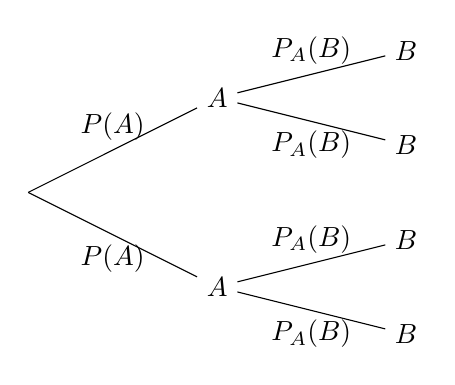
\begin{tikzpicture}[scale=1.2]
\node (A) at (2,1) {$A$};
\node (AB) at (4,1.5) {$B$};
\node (ABn) at (4,0.5) {$\overbar{B}$};
\node (An) at (2,-1) {$\overbar{A}$};
\node (AnB) at (4,-0.5) {$B$};
\node (AnBn) at (4,-1.5) {$\overbar{B}$};
\draw (0,0) -- (A) node[above,midway] {$P(A)$} -- (AB) node[midway,above] {$P_A(B)$};
\draw (A) -- (ABn) node[midway,below] {$P_A(\overbar{B})$};
\draw (0,0) -- (An) node[midway,below] {$P(\overbar{A})$} -- (AnB) node[above,midway] {$P_{\overbar{A}}(B)$};
\draw (An) -- (AnBn) node[below,midway] {$P_{\overbar{A}}(\overbar{B})$};    
\end{tikzpicture}
\end{center}
\end{example}
\begin{tcolorbox}
\begin{proposition}
\hfill
\begin{itemize}
\item Une branche de la racine à une extrémité correspond à l'intersection des événements correspondants. Pour calculer la probabilité de cette intersection, il faut multiplier les probabilités sur la branche.
\item La somme de toutes les probabilités issues d'un même noeud vaut $1$.
\item La probabilité d'un événement est égale à la somme des probabilités de toutes les branches contenant cet événement. 
\end{itemize}        
\end{proposition}
\end{tcolorbox}

% \begin{definition}
% Soit une expérience aléatoire d'univers $\Omega$. Des événements $A_1, \dots, A_k$ forment une \textbf{partition} d'$\Omega$ si et seulement si :
% \begin{itemize}
% \item Les $A_i$ sont deux à deux disjoints : il n'y a pas d'issue commune entre deux événements $A_i$.
% \item L'union $A_1 \cup \dots \cup A_k$ vaut $\Omega$ : toutes les issues possibles sont réalisées par un unique événement $A_i$.
% \end{itemize}
% \end{definition}
% \begin{center}
% \begin{tikzpicture}
% \draw (0,0) -- (5,0) -- (5,4) node[below left] {$\Omega$} -- (0,4) -- cycle;
% \draw (1,0) -- (2,4);
% \draw (3,0) -- (3,4);
% \draw (0.5,2) node {$A_1$};
% \draw (2,2) node {$A_2$};
% \draw (4,2) node {$A_3$};
% \end{tikzpicture}

% \textbf{$A_1$, $A_2$ et $A_3$ forment une partition d'$\Omega$}
% \end{center}
% \begin{remark}
% Si $A$ est un événement, alors $A$ et $\overbar{A}$ est une partition de $\Omega$.
% \end{remark}
% \begin{proposition}
% Soit $A_1, \dots, A_k$ une partition de $\Omega$, et $B$ un événement de $\Omega$. Alors, les événements $(B \cap A_1)$, \dots, $(B \cap A_k)$ sont disjoints, et 
% \begin{equation*}
% B = (B \cap A_1) \cup \dots \cup (B \cap A_k)
% \end{equation*}
% \end{proposition}
% \begin{definition}
% Un \textbf{arbre pondéré} permet de représenter plusieurs événements
% \end{definition}

\end{document}